
\begin{question}
The following figure shows a normal distribution with mean \(\mu=55\) and standard deviation \(\sigma=8\). The shaded region represents \(P(X \le 67)\) for a normally distributed random variable \(X\).\\
\pandocbounded{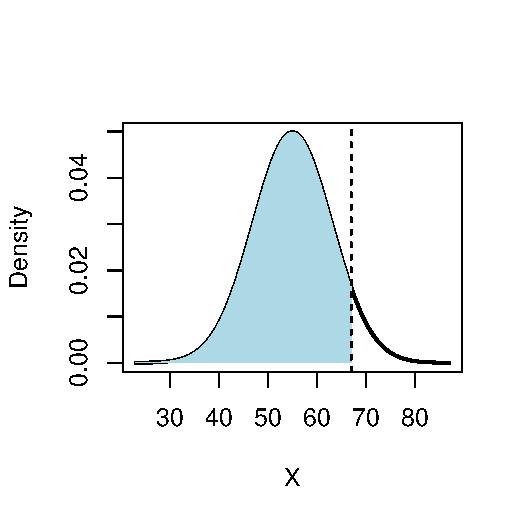
\includegraphics[keepaspectratio]{plot-1.pdf}}

Compute the probability represented by the shaded area. Round your answer to four decimal places.
\end{question}

\begin{solution}
The required probability is

\[
P(X \le 67)
=
\Phi\left(
\frac{67-55}{8}
\right).
\]

The corresponding probability is

\[
P(X \le 67) = 0.9332.
\]
\end{solution}

